The heterogen property of this 
%!TEX root = thesis.tex
% !TEX spellcheck = en-US
\chapter[Background]{Background}

\section{Energy measurement}

\section{NEON}
NEON is a general-purpose single input multiple data (SIMD) technology implemented in the ARM Cortex A series of processors.
It is able to run SIMD instructions on 128bit registers.
By utilizing the NEON unit of the ARM processors, it is possible to achive paralellism in each seperate core.
This will often open for great performance boost on problems like the ones explored in this paper.
Each register may be filled with single precission floating point numbers ranging from 8 to 64 bit each.
In future generations of the ARM ISA there will be support for other data types as well.
Different implementations of NEON exist in the Cortex A cores, and while the even the simple implementations in smaller cores like the A7 can give great performance boost, the implementations present in the newest cores are performing even better.
The A15 offer two NEON units, and the instruction pipeline to start the cores are shorter than in simpler implementations.

\section{The Performance API (PAPI)}

\section{Task based programming}
Task based programming allow a programmer to work with parallel programs, with an abstraction from the paralellization itself.
When programming with this model, the program can be split into tasks which can run in parallel.
When the program run, it will run a task manager as part of the program.
This task manager can dynamically assign tasks to the processors, and the programmer does not have to handle all the time consuming tasks related to manual parallelisation.
As long as the programmer correctly handle dependencies in the paralellized code, it will be possible to write this kind of code as if it was serial.

The task based programming model also allow simpler development of portable programs.
When the program is running tasks on available CPUs, it is not a problem to allow it to run on larger or smaller numbers of processors, and even clusters can support the program.
This model even allow the tasks to run on different types of processors in a hetrogenous enviroment.

\section[OmpSs]{OpenMP Super scalar}
OpenMP Super scalar (OmpSs) is a extention of the OpenMP API to integrate features from the StarSs programming model.
It is currently under development at the Barcelona Supercomputing Center.
The goal of OmpSs is to extend the programming model to support a wide range og processors.
The OmpSs programming model will run on a wide variety of different systems, such as traditional personal computers, clusters, shared memory systems and hetrogenous processors.
While the software is not yet comlpeted or fully tested, there have been several reports exploring it's potentilal.
The results have proven OmpSs as an efficient solution on both clusters and hetrogenous systems utilizing OpenCL and CUDA.


\section{Heterognous multi-processor}
Heterognous multi-processor systems have multiple different processors, opposed to traditional multi-processor systems.
A typical modern processor have several processors, and a program can run effectivly by having threads running parts of theis work on each of them.
This work is often of such a nature that it can run better on a different processor.
Sometimes it can run just as well on multiple simple processor, while using less die space and energy.
In other instances, an advanced processor with some special capabilities, like vector instructions, can be more efficient.

  This kind of processors have a potential to help us overcome the challenges that are emerging in processor development.
    Unfortunatly they also introduce several new challenges.

\section{Experiment platforms}

\subsection{Arendale Board} \label{ArendaleBoard}
\begin{figure}[ht!]
  \centering
  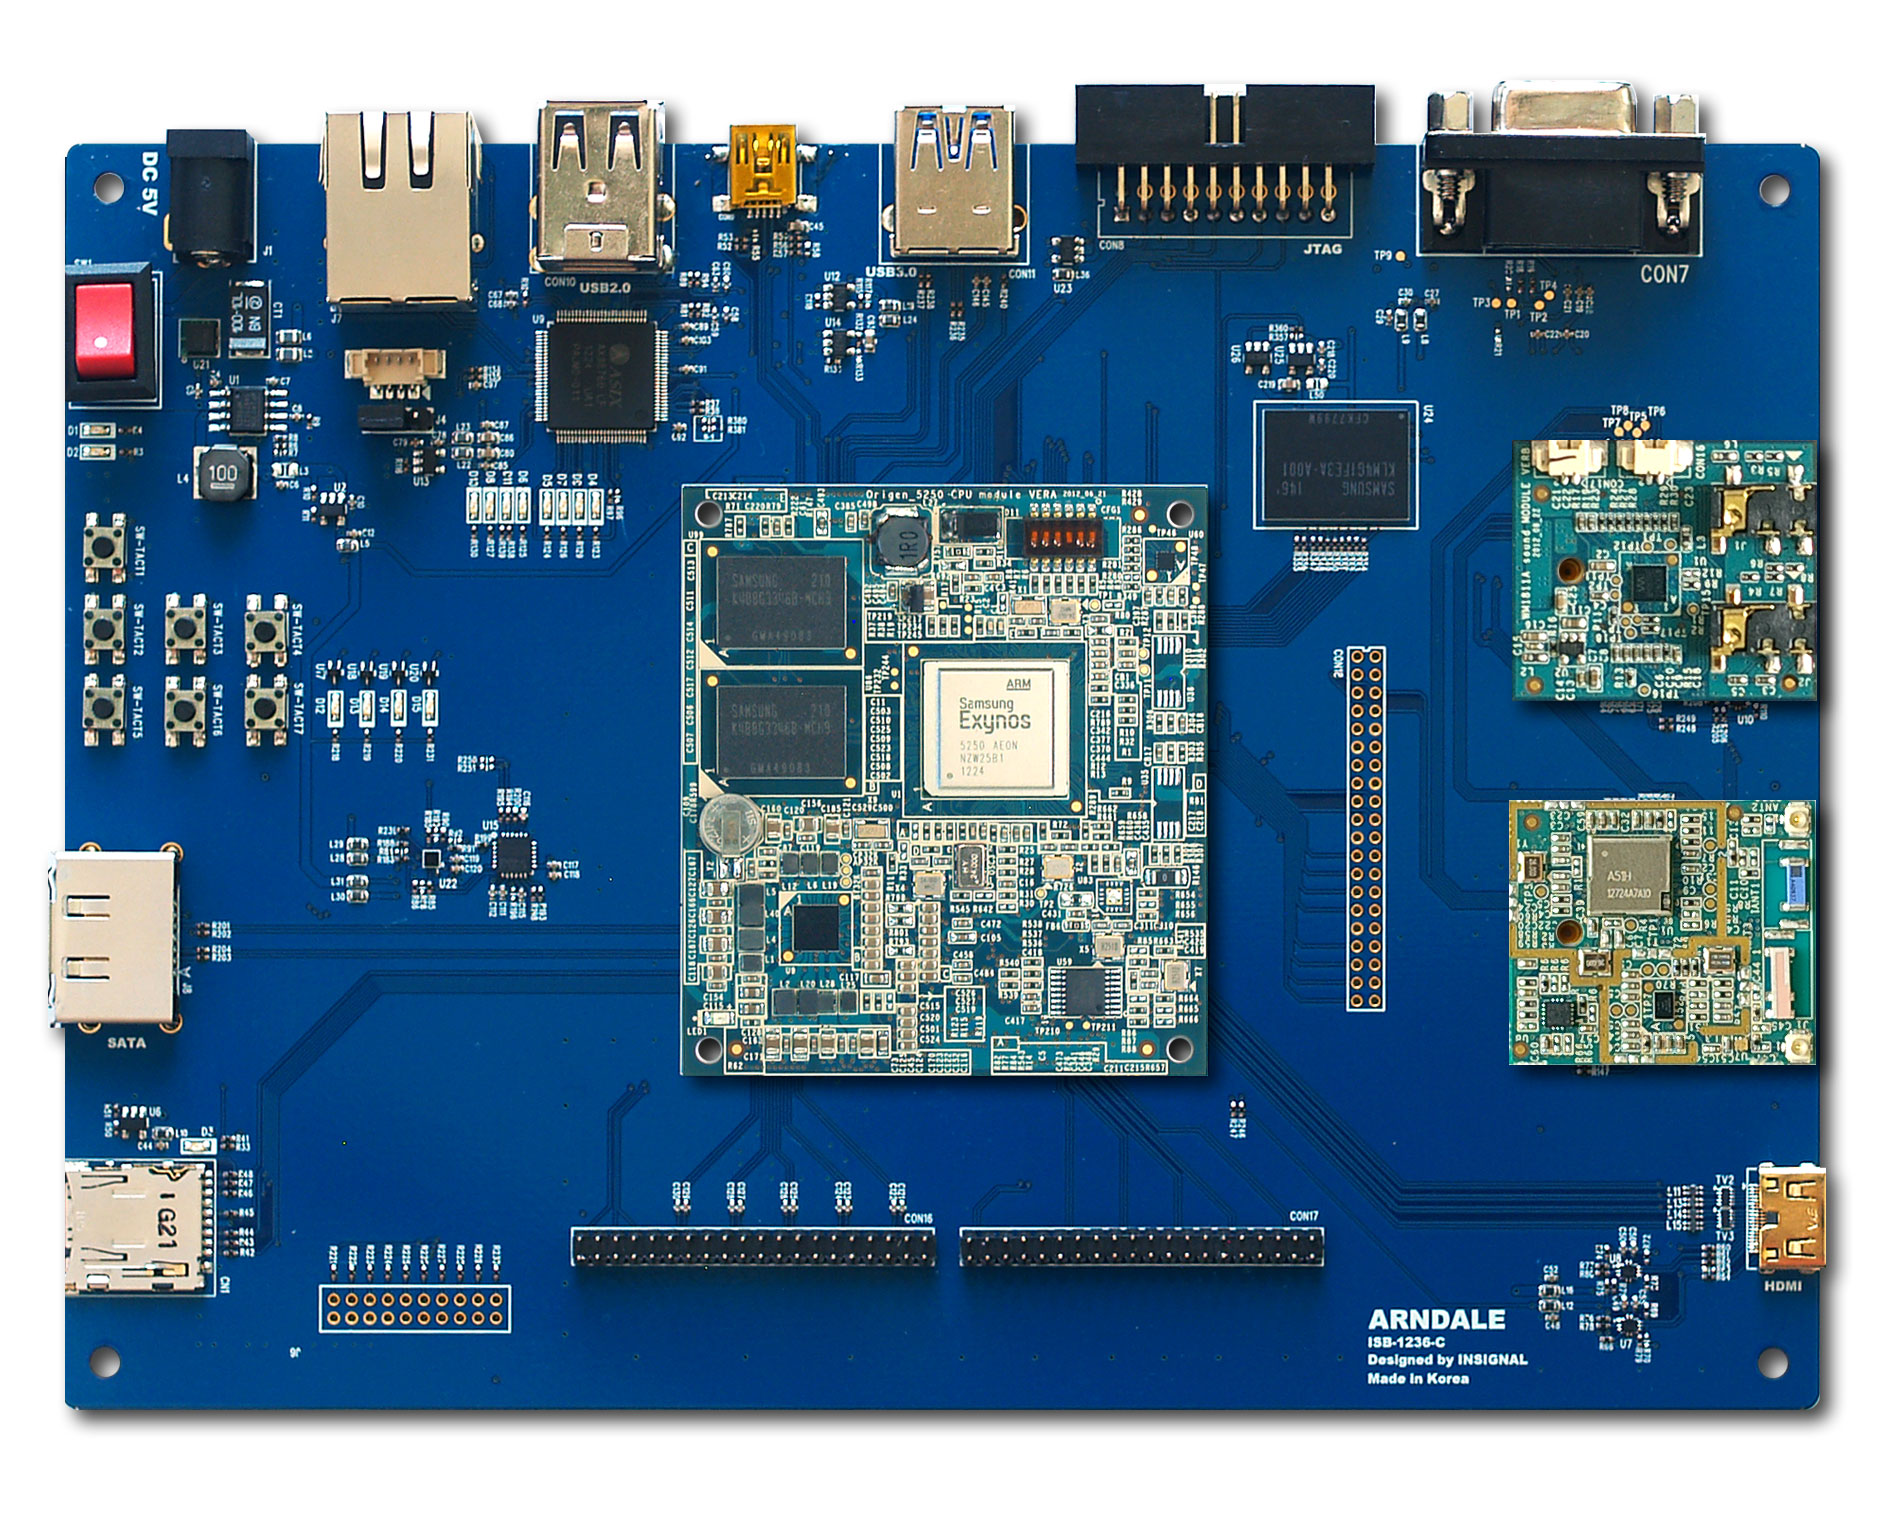
\includegraphics[width=90mm]{fig/Arendale.jpg}
  \caption{Arendale Duo \label{overflow}}
\end{figure}
The Arendale Duo is a computing system mounted on a single board.
It is fitted with an Exynos 5250 SoC, which contain a dualcore Arm Cortex-A15 , as well as an ARM Mali T-604 GPU.
This computer offer a range of supported linux distributions, as well as the OmpSs programming model.
The computer was used in the 2014 master thesis "Acceleration with OmpSs and Neon/OpenCL on ARM Processor" by Trond Inge Lillesand.
The thesis lay alot of the ground for this pilot project and planned master thesis.

\subsection{ODROID-XU3} \label{OdroidXU3}
\begin{figure}[ht!]
  \centering
  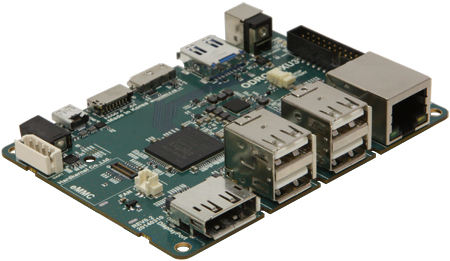
\includegraphics[width=90mm]{fig/ODROID.jpg}
  \caption{ODROID-XU3 \label{overflow}}
\end{figure}
The ODROID-XU3 is a new single-board computing system, offering interesting properties for these experiments.
The system has an Exynos 5422 heterogenous Soc.
Exynos 5422 has a quadcore ARM Cortex-A15 CPU and a ARM Mali T-628 GPU, but also a smaller quadcore ARM Cortex-A7 processor.
These 3 different processing units can be used simultaniously to solve problems.
In this paper, and the planned master thesis following it, the potency of this kind of heterogenous processor will be explored.

\subsubsection{Power monitoring}
The ODROID-XU3 commes with integrated power monitoring tools.
Implemented in hardware, it have got 4 current sensors sitting on the power pins of the Exynos SoC.
The energy monitors are indicated in figure \ref{overview-odroid}.
These monitor the current going through the large CPU cores, the small CPU cores, memory and GPU respectivly.
In addition to the current sensors, the power management for the SoC is also available to the programmer, making supply voltage to the components known.
By using the voltage and current, the power consumption is known.
As a whole, the system offer frequency, voltage, current, temperature and power readings in real time.
These fine energy and performance metrics make the system highly suitable for developers.
They are able to run their programs, collect energy profiling data and optimize their software based on the result.

\begin{figure}[ht!]
  \centering
  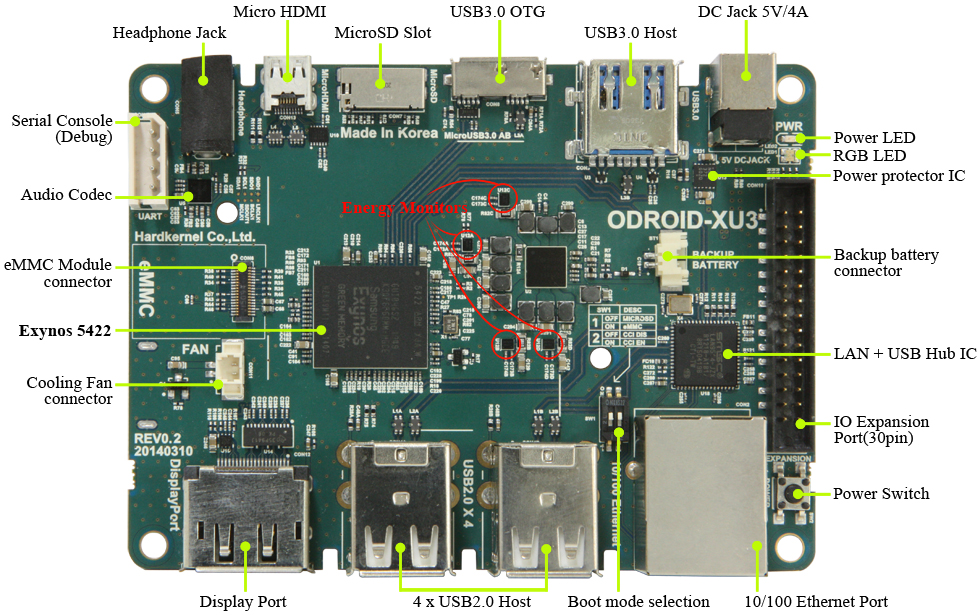
\includegraphics[width=130mm]{fig/overview-odroid.jpg}
  \caption{ODROID-XU3 anotated (hardkernel.com\cite{hardkernel01})\label{overview-odroid}}
\end{figure}
\subsubsection{Performance}

The ODROID-XU3 comes with the ARM Cortex-A15 limited to 2GHz and the ARM Cortex-A7 limited to 1.4G Hz.
There is 2GB of memory available running at 800 MHz, and the ARM Mali T-628 GPU run at 600 MHz.
This performance place it at the higher end of SoCs, but not quite in the top, as it is beaten by systems like TODO A reference system here).




TODO: Write this in a better fashion.
A key feature making this card suitable for this researchproject, is the presence of 4 seperate current sensors.
The sensors can do realtime measurement of the big CPU, little CPU, GPU and DRAM, respectivly.

\subsection{ARM Cortex-A15}
\begin{table}[H]
  \begin{tabular}{ll}
    Performance       & 1.0 GHz to 2.5GHz  \\
    L1 Cache          & 64KB \\
    L2 Cache          & 4 MB \\
    L3 Cache          & None in core, may be implemented shared in multicore system. \\
    Architecture      & ARMv7-A            \\
    Supported features& ARM Thumb-2 \\
                      & TrustZone® security technology \\
                      & NEON™ Advanced SIMD \\
                      & DSP \& SIMD extensions \\
                      & VFPv4 Floating point \\
                      & Hardware virtualization support \\
                      & Integer Divide \\
                      & Fused MAC \\
                      & Hypervisor debug instructions \\
    Memory management & 40-bit ARMv7 Memory Management Unit
  \end{tabular}
\end{table}
\subsection{ARM Cortex-A7}
The ARM Cortex-A7 is designed to be a low power alternative to the ARM Cortex-A15 and ARM Cortex-A17, with the same supported ISA and features.
This enable the ARM Cortex to be paired with it's largers relatives in a ARM big.LITTLE configuration.
\begin{table}[H]
  \begin{tabular}{ll}
    Performance       & 1.2 GHz to 1.6GHz  \\
    L1 Cache          & 8-64KB \\
    L2 Cache          & up to 1 MB \\
    L3 Cache          & None in core, may be implemented shared in multicore system. \\
    Architecture      & ARMv7-A            \\
    Supported features& ARM Thumb-2 \\
                      & TrustZone® security technology \\
                      & NEON™ Advanced SIMD \\
                      & DSP \& SIMD extensions \\
                      & VFPv4 Floating point \\
                      & Hardware virtualization support \\
                      & Integer Divide \\
                      & Fused MAC \\
                      & Hypervisor debug instructions \\
    Memory management & 40-bit ARMv7 Memory Management Unit
  \end{tabular}
\end{table}
\subsection{ARM Mali T604}
\begin{table}[H]
  \begin{tabular}{ll}
    Performance       & 533 MHz\\
                      & 17 GFLOPS  \\
    Multicore support & 1-4 cores  \\
    API Support       & OpenGL 1.1, 2.0, 3.0 and 3.1  \\
                      & OpenCL 1.1  \\
                      & DirectX 11  \\
                      & RenderScript \\
    Anti-Aliasing     & 4xFSAA with minimal performance drop  \\
                      & 16xFSAA  \\
    Cache             & 32-256KB L2 cache
  \end{tabular}
\end{table}
\subsection{ARM Mali T628}
\begin{table}[H]
  \begin{tabular}{ll}
    Performance       & 533/695 MHz \\
                      & 17/23.7 GFLOPS \\
    Multicore support & 1-8 cores  \\
    API Support       & OpenGL 1.1, 2.0, 3.0 and 3.1  \\
                      & OpenCL 1.1  \\
                      & DirectX 11  \\
                      & RenderScript \\
    Anti-Aliasing     & 4xFSAA with minimal performance drop  \\
                      & 16xFSAA  \\
    Cache             & 32-256KB L2 cache
  \end{tabular}
\end{table}

\section{Algorithms}
Here I will write about the algorithms used in the experiments.

